 % The main file for CAMP reports
 % Don't put any content in here. 
 % Don't even include content files by using \input or \inlcude. 
 % Put your content to TEXT.TEX or include it there using \input.
 % Uses:
 %		SETTINGS.TEX	contains the settings for this document
 %		COMMANDS.TEX	contains commands which can be used while writing
 %		INFO.TEX			contains the author, title and so on for the cover
 %		COVER.TEX			formats the front cover of the document
 %		ABSTRACT.TEX	contains the abstract to be included (if needed)
 %		TEXT.TEX			contains the actual content of the document
 %		BIB.BIB				containt the BibTeX entries for the document
 
 
%% Draft document mode
%% Final document
\documentclass[11pt,a4paper,bibtotoc,idxtotoc,headsepline,footsepline,footexclude,BCOR12mm,DIV13]{scrbook}

%\documentclass[11pt,a4paper,bibtotoc,idxtotoc,headsepline,footsepline,footexclude,BCOR20mm,DIV10]{scrbook}

% KOMA-Optionen:
%  bibtotoc: include bibliography in table of contents
%  idxtotoc: include index in table of contents
%  headsepline: use horizontalline under heading
%  BCOR: binding correcion (Bindungskorrektur) (e.g.: BCOR5mm)
%  DIV: Number of sheet sections (used for layout) (e.g.: DIV12) 



% include title and author information for the cover
% Set here the title, authors and other stuff to be used for the cover
% This file is used by MAIN.TEX

% set title, authors and stuff for the cover
\def\doctype{Mater's Thesis in Biomedical Computing}
\def\title{The Big Work - Deformable object detection in underwater imaging}
\def\titleGer{Deformierbare Objekterkennung in Unterwasser-Bilder}
\def\author{Andr\'es S\'anchez}
\def\date{November 27, 2013}

% text to appear in the footer
\def\footertext{}

% include settings
% Included by MAIN.TEX
% Defines the settings for the CAMP report document

\renewcommand{\sectfont}{\normalfont \bfseries}        % Schriftart der Kopfzeile

% manipulate footer
\usepackage{scrpage2}
\pagestyle{scrheadings}
\ifoot[\footertext]{\footertext} % \footertext set in INFO.TEX
%\setkomafont{pagehead}{\normalfont\rmfamily}
\setkomafont{pagenumber}{\normalfont\rmfamily}

%% allow sophisticated control structures
\usepackage{ifthen}

% use Palatino as default font
\usepackage{palatino}

% enable special PostScript fonts
\usepackage{pifont}

% make thumbnails
\usepackage{thumbpdf}

%to use the subfigures
\usepackage{subfigure}
% \usepackage{subfig}


\usepackage{colortbl}



%% show program code\ldots
%\usepackage{verbatim}
% \usepackage{program}

%% enable TUM symbols on title page
\usepackage{styles/tumlogo}


\usepackage{multirow}

%% use colors
\usepackage{color}

%% make fancy math
\usepackage{amsmath}
\usepackage{amsfonts}
\usepackage{amssymb}
\usepackage{textcomp}
\usepackage{yhmath} % f�r die adots 
%% mark text as preliminary
%\usepackage[draft,german,scrtime]{prelim2e}

%to add seudo algorithm
% \usepackage{algorithm}
\usepackage{algorithm2e}

%% create an index
\usepackage{makeidx}

% for the program environment
\usepackage{float}

%% load german babel package for german abstract
%\usepackage[german,american]{babel}	
\usepackage[german,english]{babel}
\selectlanguage{english}

% use german characters as well
\usepackage[latin1]{inputenc}       % allow Latin1 characters

% use initals dropped caps - doesn't work with PDF
% drop Cap superseded by lettrine package
% \usepackage{dropping}
\usepackage{lettrine}


\usepackage{styles/shortoverview}
%----------------------------------------------------
%      Graphics and Hyperlinks
%----------------------------------------------------

%% check for pdfTeX
\ifx\pdftexversion\undefined
 %% use PostScript graphics
 \usepackage[dvips]{graphicx}
 \DeclareGraphicsExtensions{.eps,.epsi,.png}
 \graphicspath{{figures/}{figures}} 

 %to add todo notes
 \usepackage{todonotes}

 %% allow rotations
 \usepackage{rotating}
 %% mark pages as draft copies
 %\usepackage[english,all,light]{draftcopy}
 %% use hypertex version of hyperref
 \usepackage[hypertex,hyperindex=false,colorlinks=false]{hyperref}
\else %% reduce output size \pdfcompresslevel=9
 %% declare pdfinfo
 %\pdfinfo { 
 %  /Title (my title) 
 %  /Creator (pdfLaTeX) 
 %  /Author (my name) 
 %  /Subject (my subject	) 
 %  /Keywords (my keywords)
 %}
 %% use pdf or jpg graphics
 \usepackage[pdftex]{graphicx}
 \DeclareGraphicsExtensions{.jpg,.JPG,.png,.pdf,.eps}
 \graphicspath{{figures/}} 

 %to add todo notes
 \usepackage{todonotes} 

 %to modify margin wjen needed it
 \usepackage{chngpage} 


 %% Load float package, for enabling floating extensions
 \usepackage{float}
 
 %% allow rotations
 \usepackage{rotating}
 %% use pdftex version of hyperref
 \usepackage[pdftex,colorlinks=true,linkcolor=red,citecolor=red,%
 anchorcolor=red,urlcolor=red,bookmarks=true,%
 bookmarksopen=true,bookmarksopenlevel=0,plainpages=false%
 bookmarksnumbered=true,hyperindex=false,pdfstartview=%
 ]{hyperref}
%
%\usepackage[pdftex,colorlinks=false,linkcolor=red,citecolor=red,%
% anchorcolor=red,urlcolor=red,bookmarks=true,%
% bookmarksopen=true,bookmarksopenlevel=0,plainpages=false%
% bookmarksnumbered=true,hyperindex=false,pdfstartview=%
% ]{hyperref}
\fi




%% Fancy chapters
%\usepackage[Lenny]{fncychap}
%\usepackage[Glenn]{fncychap}
%\usepackage[Bjarne]{fncychap}

%\usepackage[avantgarde]{quotchap}
\usepackage[square]{natbib}

% set the bibliography style
%\bibliographystyle{styles/bauermaNum}
% \bibliographystyle{alpha}
\bibliographystyle{plainnat}

% include commands
% Commands to be used within the TUM report document
% Included by MAIN.TEX
% Please include your own cool commands here. 
% Be only sure to comment it sufficiently so others can use it.

%-------------------------------------------------------------
%                      Own Commands
%-------------------------------------------------------------


%-------------------------------------------------------------
% math stuff -------------------------------------------------

% nice R, N, C
\newcommand{\nat}{\mathbb{N}}
\newcommand{\real}{\mathbb{R}}
\newcommand{\compl}{\mathbb{C}}



% norm
\newcommand{\norm}[1]{\left\| #1 \right\|}

% un demi
\newcommand{\half}{\frac{1}{2}}

% parantheses
\newcommand{\parenth}[1]{ \left( #1 \right) }
\newcommand{\bracket}[1]{ \left[ #1 \right] }
\newcommand{\accolade}[1]{ \left\{ #1 \right\} }
%\newcommand{\angle}[1]{ \left\langle  #1 \right\rangle }

% partial derivative: %#1 function, #2 which variable
% simple / single line version
\newcommand{\pardevS}[2]{ \delta_{#1} f(#2) }
% fraction version
\newcommand{\pardevF}[2]{ \frac{\partial #1}{\partial #2} }

% render vectors: 3 and 4 dimensional
\newcommand{\veciii}[3]{\left[ \begin{array}[h]{c} #1 \\ #2 \\ #3	\end{array} \right]}
\newcommand{\veciv}[4]{\left[ \begin{array}[h]{c} #1 \\ #2 \\ #3 \\ #4	\end{array} \right]}

% render matrices: 3  dimensional (arguments in row first order)
\newcommand{\matiii}[9]{\left[ \begin{array}[h]{ccc} #1 & #2 & #3 \\ #4 & #5 & #6 \\ #7 & #8 & #9	\end{array} \right]}
%DOESN'T WORK,DON'T KNOW WHY \newcommand{\mativ}[16]{\left[ \begin{array}[h]{cccc} #1 & #2 & #3 & #4 \\ #5 & #6 & #7 & #8 \\ #9 & #10 & #11 & #12 \\ #13 & #14 & #15 & #16 \end{array} \right]}


%-------------------------------------------------------------
%-------------------------------------------------------------


%-------------------------------------------------------------
% some abreviations ------------------------------------------
\newcommand{\Reg}{$^{\textregistered}$}
\newcommand{\reg}{$^{\textregistered}$ }
\newcommand{\Tm}{\texttrademark}
\newcommand{\tm}{\texttrademark~}
\newcommand {\bsl} {$\backslash$}

%-------------------------------------------------------------
%-------------------------------------------------------------


%-------------------------------------------------------------
% formating --------------------------------------------------

% Theorem & Co environments and counters
\newtheorem{theorem}{Theorem}[chapter]
\newtheorem{lemma}[theorem]{Lemma}
\newtheorem{corollary}[theorem]{Corollary}
\newtheorem{remark}[theorem]{Remark}
\newtheorem{definition}[theorem]{Definition}
\newtheorem{equat}[theorem]{Equation}
\newtheorem{example}[theorem]{Example}
% \newtheorem{algorithm}[theorem]{Algorithm}

% inserting figures
\newcommand{\insertfigure}[4]{ % Filename, Caption, Label, Width percent of textwidth
	\begin{figure}[htbp]
		\begin{center}
			\includegraphics[width=#4\textwidth]{#1}
		\end{center}
		\vspace{-0.4cm}
		\caption{#2}
		\label{#3}
	\end{figure}
}




% referecing figures

\newcommand{\refFigure}[1]{ %label
	figure \ref{#1}
}
\newcommand{\refChapter}[1]{ %label
	chapter \ref{#1}
}

\newcommand{\refSection}[1]{ %label
	section \ref{#1}
}

\newcommand{\refParagraph}[1]{ %label
	paragraph \ref{#1}
}

\newcommand{\refEquation}[1]{ %label
	equation \ref{#1}
}

\newcommand{\refTable}[1]{ %label
	table \ref{#1}
}




\newcommand{\rigidTransform}[2]
{
	${}^{#2}\!\mathbf{H}_{#1}$
}

%code, in typewriter
\newcommand{\code}[1]
 {\texttt{#1}}

% comment that appears on the border - very practical !!!
\newcommand{\comment}[1]{\marginpar{\raggedright \noindent \footnotesize {\sl #1} }}

% page clearing
\newcommand{\clearemptydoublepage}{%
  \ifthenelse{\boolean{@twoside}}{\newpage{\pagestyle{empty}\cleardoublepage}}%
  {\clearpage}}


%-------------------------------------------------------------
%-------------------------------------------------------------


\newcommand{\etAl}{\emph{et al.}\mbox{ }}


%\makeindex
	%% inter line spacing
%\linespread{1.0}

\makeglossary

\begin{document}

	\frontmatter
	
	
	% The front cover for the TUM report document.
% Included by MAIN.TEX


%--------------------------------------------------
% The Front Cover
%--------------------------------------------------

% The front cover for the TUM document.
% Included by MAIN.TEX


%--------------------------------------------------
% The Front Cover
%--------------------------------------------------

% correct BCOR - undo at the end !!!
\def\bcorcor{0.15cm}
\addtolength{\hoffset}{\bcorcor}

\thispagestyle{empty}

 \vspace{4cm}
\begin{center}
	       \oTUM{4cm}
	   
	   \vspace{5mm}     
	   \huge FAKULT{\"A}T F{\"U}R INFORMATIK\\ 
	   \vspace{0.5cm}
	 \large DER TECHNISCHEN UNIVERSIT{\"A}T M{\"U}NCHEN\\
    \vspace{1mm}
        
	\end{center}
		

\vspace{15mm}
\begin{center}

   {\Large \doctype}

  \vspace{20mm}
  
  {\huge\bf \title}\\%[3ex]
  
  
  \vspace{15mm}
  
  
  {\LARGE  \author}
  
  \vspace{10mm}
  
  \begin{figure}[h!]
  \centering
   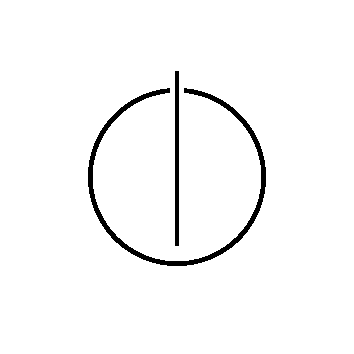
\includegraphics[width=4cm]{styles/informat.png}
  \end{figure}
  
  \end{center}
%	\clearemptydoublepage
%	
%	% The titlepage for the CAMP report document.
% Included by MAIN.TEX


%--------------------------------------------------
% The title page
%--------------------------------------------------

% correct BCOR - undo at the end !!!
\def\bcorcor{0.15cm}
\addtolength{\hoffset}{\bcorcor}

\thispagestyle{empty}

 \vspace{10mm}
\begin{center}
	       \oTUM{4cm}
	   
	   \vspace{5mm}     
	   \huge FAKULT{\"A}T F{\"U}R INFORMATIK\\ 
	   \vspace{0.5cm}
	 \large DER TECHNISCHEN UNIVERSIT{\"A}T M{\"U}NCHEN\\
        
	\end{center}
		

\vspace{10mm}
\begin{center}

   {\Large \doctype}

  \vspace{10mm}
  
  {\LARGE \title}\\
  
  
  \vspace{10mm}
  
  
  {\LARGE  \titleGer}\\
  
  
  \vspace{10mm}

    %\hfill
    \begin{tabular}{ll}
	   \Large Author:     & \Large \author \\[2mm]
	   \Large Examiner:    & \Large Prof. Dr. Nassir Navab \\[2mm]				
	   \Large Supervisor:    & \Large Prof. Dr. Slobodan Ilic \\[2mm]				
	   \Large Advisor:	& \Large M.Sc. David J. Tan \\[2mm]
	   \Large Date:       & \Large November 27, 2013
	 \end{tabular}
	 
	 \vspace{5mm}
	 
	 \begin{figure}[h!]
  \centering
   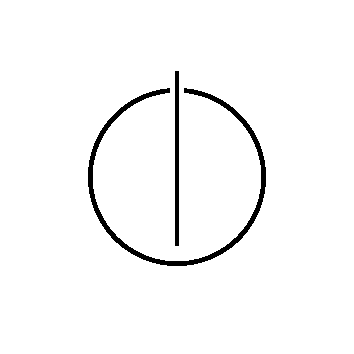
\includegraphics[width=4cm]{styles/informat.png}
  \end{figure}
   

\end{center}

% undo BCOR correction
\addtolength{\hoffset}{\bcorcor}

	
	
%	\input{components/cover_maschmeyer}
	\clearemptydoublepage
	
	% The titlepage for the CAMP report document.
% Included by MAIN.TEX


%--------------------------------------------------
% The title page
%--------------------------------------------------

% correct BCOR - undo at the end !!!
\def\bcorcor{0.15cm}
\addtolength{\hoffset}{\bcorcor}

\thispagestyle{empty}

 \vspace{10mm}
\begin{center}
	       \oTUM{4cm}
	   
	   \vspace{5mm}     
	   \huge FAKULT{\"A}T F{\"U}R INFORMATIK\\ 
	   \vspace{0.5cm}
	 \large DER TECHNISCHEN UNIVERSIT{\"A}T M{\"U}NCHEN\\
        
	\end{center}
		

\vspace{10mm}
\begin{center}

   {\Large \doctype}

  \vspace{10mm}
  
  {\LARGE \title}\\
  
  
  \vspace{10mm}
  
  
  {\LARGE  \titleGer}\\
  
  
  \vspace{10mm}

    %\hfill
    \begin{tabular}{ll}
	   \Large Author:     & \Large \author \\[2mm]
	   \Large Examiner:    & \Large Prof. Dr. Nassir Navab \\[2mm]				
	   \Large Supervisor:    & \Large Prof. Dr. Slobodan Ilic \\[2mm]				
	   \Large Advisor:	& \Large M.Sc. David J. Tan \\[2mm]
	   \Large Date:       & \Large November 27, 2013
	 \end{tabular}
	 
	 \vspace{5mm}
	 
	 \begin{figure}[h!]
  \centering
   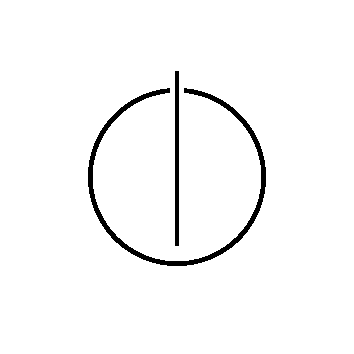
\includegraphics[width=4cm]{styles/informat.png}
  \end{figure}
   

\end{center}

% undo BCOR correction
\addtolength{\hoffset}{\bcorcor}

	
	
	\clearemptydoublepage


\thispagestyle{empty}
\selectlanguage{german}
	\vspace*{0.8\textheight}
	\noindent
	Ich versichere, dass ich diese Diplomarbeit selbst{\"a}ndig verfasst und nur 
	die angegebenen \\Quellen und Hilfsmittel verwendet habe.
	
	\vspace{15mm}
	\noindent
	M{\"u}nchen, den \today \hspace{5cm} \author
\selectlanguage{english}
\newpage
	
	\clearemptydoublepage
\phantomsection
\addcontentsline{toc}{chapter}{Acknowledgements}	


%\chapter*{Acknowledgements}

\vspace*{2cm}

\begin{center}
{\Large \bf Acknowledgments}
\end{center}

\vspace{1cm}




If someone contributed to the thesis... might be good to thank them here.
to the person that support me all the time, My lovely Wife Karin, who understand me
almost always
	
	% Abstract for the TUM report document
% Included by MAIN.TEX


\clearemptydoublepage
\phantomsection
\addcontentsline{toc}{chapter}{Abstract}	





\vspace*{2cm}
\begin{center}
{\Large \bf Abstract}
\end{center}
\vspace{1cm}

An abstracts abstracts the thesis!

	\tableofcontents
  
  \clearemptydoublepage

\phantomsection
\addcontentsline{toc}{chapter}{Outline of the Thesis}

\begin{center}
	\huge{Outline of the Thesis}
\end{center}




%--------------------------------------------------------------------
\section*{Part I: Introduction and Theory}

\noindent {\scshape Chapter 1: Introduction}  \vspace{1mm}

\noindent  This chapter presents an overview of the thesis and it purpose. Furthermore, it will discuss the sense of life in a very general approach.  \\

\noindent {\scshape Chapter 2: Theory}  \vspace{1mm}

\noindent  No thesis without theory.   \\

%--------------------------------------------------------------------
\section*{Part II: The Real Work}

\noindent {\scshape Chapter 3: Overview}  \vspace{1mm}

\noindent  This chapter presents the requirements for the process.

	\mainmatter
	
	
		% ---------------------------------------------------------------------------
		%
		%Introduction and Background Theory
		%
		% ---------------------------------------------------------------------------
		\part[Introduction and Theory]{Introduction and Theory}
		\label{part:introAndBackgroundTheory}
		\chapter{Introduction}
\label{chapter:Introduction}



% Here starts the thesis with an introduction. Please use nice latex and bibtex entries \cite{latex}. Do not spend time on formating your thesis, but on its content. 
 
\section{Motivation}
As we progress from livelihood fisheries to aquaculture industries, the global 
production and demand of fishes has drastically increased over several decades. 
According to \cite{Asche2011}, the production increased from 16 M in the 1970s to 
142 M in 2008. In these statistical figures, the amount if wild fishes has reached 
a threshold since 1980s while the farmed fishes picked up the difference in amount.
For instance, \citeauthor{LARSEN2011a} mention in \citeyearpar{LARSEN2011a} that Norway 
alone increased their production of Salmons from a few thousand in the 1980s to 
approximately 1.4 M in 2009 which constitutes around 51\% of the global supply. 
This makes then the largest supplier of Salmons in the world \citep{Asche2011, LARSEN2011a, Liu2011}.

Other than favourable geographical and environmental features that made Norway viable 
for this industry technological advancement also played an important role in the 
economical cycle between demand and supply. As production increase, they reduced 
cost and as a consequence, increased the demand \cite{Asche2011}. Therefore, this cycle 
supported the growth of the industry over the years.
Since around, 80 \% of all sales of farmed fish are arranged pre-harvest, the profit 
on the sale directly depends on the correct estimations of weight, size distribution 
and total biomass. Therefore, our project deals with remote monitoring of fishes size 
and weight distribution in aquaculture environments. Considering a large amount of fish, 
it becomes essential to develop an automated biomass estimator to constantly monitor 
the changes or growth of fishes. This system involves cameras that would detect the 
fish in a video sequence and compute the biomass distribution over a specified period 
of time.
\todo {Add description of hardware setup}

\todo { check this paragraph}
% Underwater stereo-video measurement systems are used widely for counting
% and measuring fish in aquaculture, fisheries and conservation management.
% To determine population counts, spatial or temporal frequencies, most commonly
%  using a point and click process by human operator.
% Current research aims to use stereo 3d depth vision system. 
% A fully automated process will require the detection and identification
% of candidates for measurement, followed by the SNOUT to fork length measurement, 
% as well as the counting and tracking of fish. This Thesis present a review and 
% implementation of techniques uses for the detection, Identification, measurement, 
% counting and tracking of fish in underwater image sequences, including consideration 
% of the changing in body shape.
% The review will analyse the most commonly used approaches, leading to an evaluation 
% of techniques most likely to be a  general solution to the complete process of 
% detection, measurement, counting and tracking


\section{Problem Statement}

This work is part of the project call fishscan, where the main goal is design a 
system for remote monitoring of fishes size and weight distribution in aquaculture 
environments. during this project was develop a camera rig system consist in a 
underwater housing with a time of flight camera with LED light source and a 2D CCD 
grayscale camera as is shown in the fig \ref{fig:rigsetup}.

\begin{figure}[h]
\centering
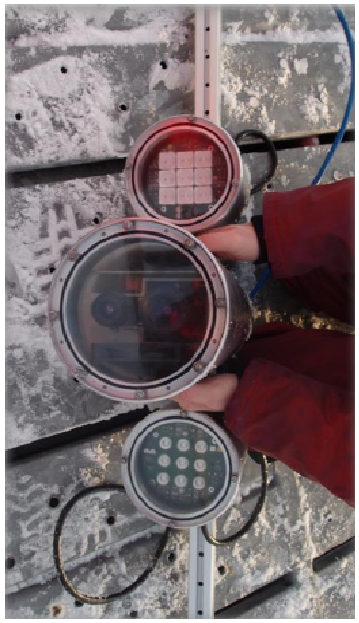
\includegraphics[scale=0.4]{rigsetup}
\caption{Rig Camera System - TOF + CCD cameras}
\label{fig:rigsetup}
\end{figure}


as the main goal of the project is compute the biomass of the fish by computing 
the volume of it, taken the concept of mass density from the physics, using the relation
between biomass and volume. Then, this problem of biomass estimation can be formulated
as a problem of volume estimation of the fish. to achieve this objective, the first 
step is the fish detection in an 2D grayscale image. followed by a back-projection 
into the TOF image where the is possible to fit a 3D model to the detected fish.
it is important to mention that the approach assume in this work is due of highly 
noisy image acquire by the range imaging camera, which was adapted to work in a 
underwater environment, but as you can see in the 3D image shown in \ref{fig:tofNoisy}


\begin{figure}[h]
\centering
\subfigure[Intensity Image TOF camera]{
	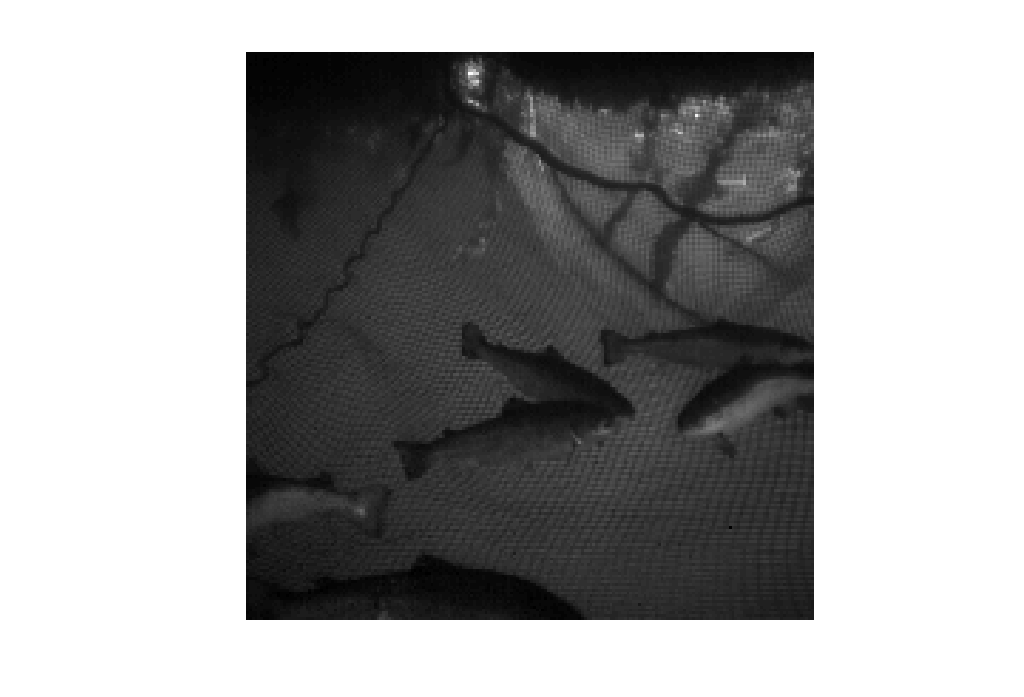
\includegraphics[scale=0.3]{tof_1}
}\subfigure[depth Image]{
	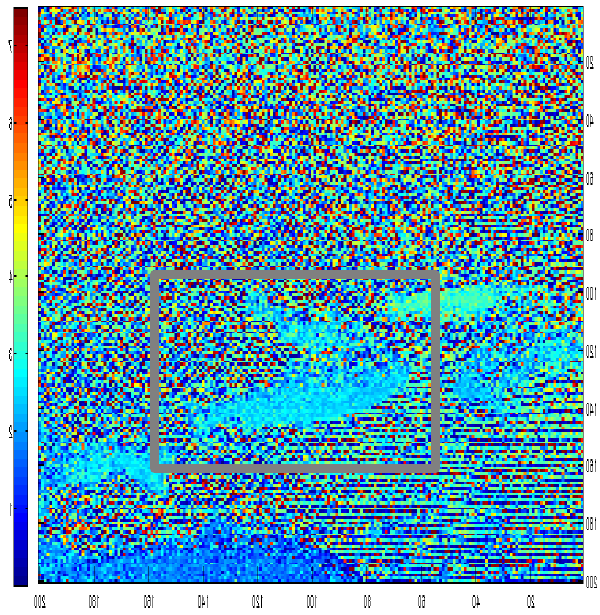
\includegraphics[scale=0.3]{tof_2}
}
% \qquad
\subfigure[3D represemtation depth image]{
	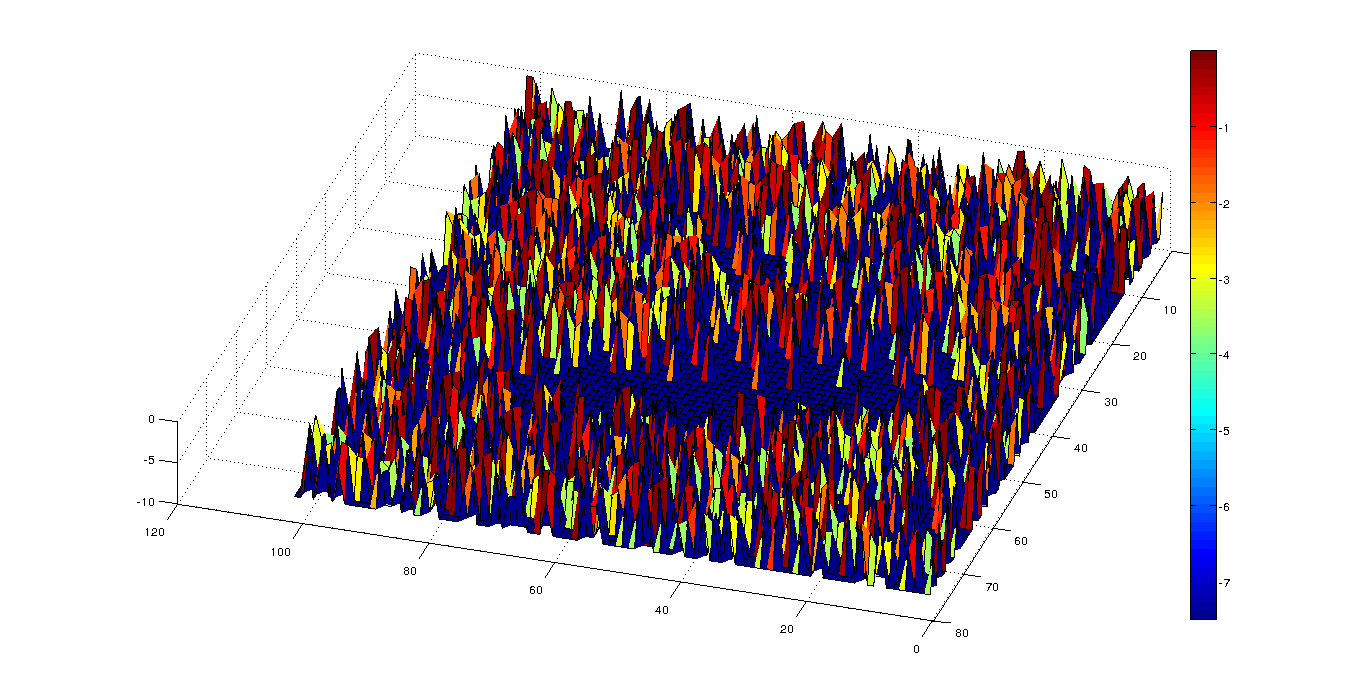
\includegraphics[scale=0.3]{tof_3}
}%
\caption{TOF camera images.}
\label{fig:tofNoisy}
\end{figure}

although, the detection using the 2D intensity image alone cannot compute the volume
of the fish because it is not depth invariant and the size is up-to-scale; This work 
will may use of the 2D intensity image as a First step, detecting the fish contour.
The pipeline depicted in \todo{ add image ref \ref{}} consist of three major steps
that are: fish detection, contour extraction, volume-biomass estimation. In this 
project, we concentrate on the first step that is fish detection and contour extraction.

At this point we need to find a algorithm for fish detection and contour extraction 
that addresses the three major challenges of our problem, These are:

\begin{enumerate}
\item \textit{Deformations}, THe algorithm must handle different motions of the
which suggests that we are dealing with a deformable (articulated) object.
\item \textit{Different Viewpoints}, As the fish move around its environment, the 
algorithm must be able to detect the fish from different perspectives.
\item \textit{Occlusions}, The algorithm must also be able to handle occlusion, 
e.g. self occlusions, occlusion from another fishes and occlusion from object in 
the environment.
\end{enumerate}

Based on the three challenges and the use of 2D intensity values obtained from the
2D CCD camera, we propose an approach inspired by two works from, the first, 
\citet{Mixtures-of-parts} which describe a method for articulated human detection
and human pose estimation in static images based on a representation of deformable 
part models. The main idea of their approach is to use a mixture of small, non-oriented 
parts, which describe a general, flexible mixture model that jointly captures spatial 
relations between parts locations and co-occurrences relations between part mixtures, 
augmenting standard pictorial structure models that encode just spatial relations. 
The second approach is propose in \citet{Hinterstoisser2012}, where they present 
a method for real-time 3D object instance detection that does not require a time 
consuming training stage, and can handle untextured objects. At its core, the approach 
presented is a novel image representation for template matching designed to be robust 
to small image transformations, This robustness is based on spread image gradient 
orientations and allows to test only a small subset of all possible pixel locations 
when parsing a image.
In our approach, that can be considerer in the groups of machine learning method, 
the learning process process tries to understand the relation between the input $X$
and output $Y$; such that when the input $X$ is given, it can predict the outcome $Y$.
In our case, the input $X$ are 2D grayscale intensity image containing fishes under
different deformations and seen from different perspectives, while the expected output
$Y$ are the positions of the desired keypoints and corresponding contours for the detected
fishes, However, in the learning stage, we require a large amount of data that shows
this relations. We need a great amount of labeled 2D intensity image where the locations
of the keypoints and contours are given. unfortunately, the current motion tracking systems
from human pose estimation are not a valid solution to find ground truth data for fish
because the difference in behaviour as well as the difference in environment.Therefore,
we address this problem by hand labeling real 2D deformed fishes images of a group of in a real
scenario, where the fish are observed from different perspectives.

\todo{ add short description of learning stage for part based and linemod}


We evaluate the proposed method by matching the \todo{explain method the evaluate result}

Therefore, this thesis accomplished the following: create a labeled real fish images datasets
that comprise of intensity images acquire by 2D CCD camera, learn esqueleton and countours from
labeled datasets, predict keypoints and contours an unlabeled 2D fish images and verify the validality
of the predictions that will be discussed in Chapter 3 \todo{add ref}. A overview
of the related works is in Chapter 2 \todo{add ref} while the implementations details are
presented in Chapter 4. The result is discussed in Chapter 5 and finally, we conclude in Chapter 6.

\todo { Continue from here}

% The monitoring of fish for stock assessment in aquaculture,
% commercial fisheries and in the assessment of the effectiveness of biodiversity 
% management strategies such as Marine Protected Areas and closed area management 
% is essential for the economic and environmental management of fish population,
% Video based techniques for fishery independent and non-destructive sampling now 
% widely accepted.
% The advantages of suing stereo-video for counting the numbers of fish. measuring 
% their length and defining the sample area have been well demonstrated.
% However, the time lag and cost of processing video imagery decreases the cost of 
% effectiveness and uptake of this technology. Current research aims t
	


% \section{Next Section}
% There is no need for a latex introduction since there is plenty of literature out there.

		
		
		%
		%% ---------------------------------------------------------------------------
		%%
		%% Fully Automated Calibration for Ultrasound
		%%
		%%% ---------------------------------------------------------------------------
		\part[The 2nd Part]{The Second Part}
		\label{part:secondP}
		
		
		% ---------------------------------------------------------------------------
		%
		% Appendix
		%
		% ---------------------------------------------------------------------------
		
		\part*{Appendix}
		\addcontentsline{toc}{part}{Appendix}
		
		\appendix %---------------------------------------
		
		\chapter{Detailed Descriptions}
%\section{Detailed Validation Results}
\label{chapter:DetailedDescriptions}
Here come the details that are not supposed to be in the regular text.
		
	


  \clearemptydoublepage
  
	\bibliography{bibliography/literature}
	
 
\end{document}

